% !TEX encoding = UTF-8 Unicode 
% !TEX root = praca.tex

\chapter{Opis systemu}

Rozdział ten poglądowo opisuje system będący przedmiotem pracy, z naciskiem na 
architekturę oprogramowania i projektowanie systemów. 
Poszczególne elementy systemu zostały przedstawione na schemacie poglądowym na rys. \ref{fig:hl_sys}.

\begin{figure}[h!]
    \centering
    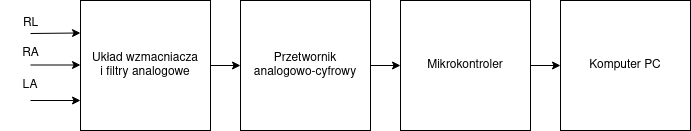
\includegraphics[scale=0.6]{pl/media/hl_system.png}
    \caption{Schemat poglądowy systemu}
    \label{fig:hl_sys}
\end{figure}

Do pomiaru aktywności elektrycznej serca zastosowano klasyczny układ 3 elektrod pomiarowych używany często
w diagnostyce arytmii \cite{FRANCIS201692}, z oznaczeniami \textit{RL} (\textit{right leg}, prawa noga), 
\textit{RA} (\textit{right arm}, prawa ręka) oraz \textit{LA} (\textit{left arm}, lewa ręka). W tej 
konfiguracji elektrody można umieścić w sposób jaki sugerują oznaczenia tzn. na kończynach lub alternatywnie 
na klatce piersiowej (\textit{RA} i \textit{LA}) oraz poniżej żeber (\textit{RL}). 
Istnieje możliwość zmiany umiejscowienia elektrod tak aby utworzyć inne konfiguracje, które również umożliwiają akwizycję sygnału
mającego wartość w diagnostyce chorób serca.

\begin{figure}[h!]
    \centering 
    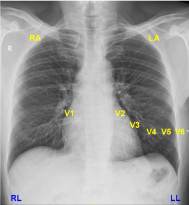
\includegraphics[scale=1.2]{pl/media/electrodes.png}
    \caption{Zdjęcie rentgenowskie klatki piersiowej wraz z oznaczeniami\\ dla 3-elektrodowej konfiguracji oraz oznaczeniami dodatkowymi
    \cite{FRANCIS201692}(\textit{Fig. 1.})}
    \label{fig:ele}
\end{figure}

\newpage

\section{Wzmocnienie sygnału i filtracja analogowa}

Sygnał \textit{EKG} charakteryzuje się małymi amplitudami, w zakresie od dziesiątek do setek $\mu V$ \cite{Zywietz1990}.
Ta cecha badanego sygnału uniemożliwia dokonywanie pomiaru w sposób dokładny przez klasyczne przetworniki analogowo/cyfrowe (\textit{ADC}, \textit{Analog to Digital Converter})
ze względu na ich niską rozdzielczość. Jako rozwiązanie w pracy zastosowano zestaw wzmacniaczy w układzie scalonym firmy \textit{Analog Devices}, \textit{AD8232} \cite{AD8232ds}. 
Ze względu na to że mierzone impulsy mogą mieć wartości ujemne, \textit{AD8232} przesuwa wzmacnia i normalizuje amplitudę sygnału do przedziału $[0; 3,3V]$ co umożliwia 
próbkowanie i jego kwantyzację za pomocą klasycznych przetworników \textit{ADC}. 
\textit{AD8232} zapewnia również mechanizm wykrywania podłączonych elektrod (ang. \textit{leads off detection}).


W pracy użyto płytki drukowanej z układem \textit{AD8232} \cite{AD8232BS} w konfiguracji z dwoma pasywnymi filtrami analogowymi: 
górnoprzepustowym oraz dolnoprzepustowym, o wynikowym paśmie przepuszczania $[0,5 Hz; 40Hz]$ (rys. \ref{fig:afilt}) \cite{AD8232ds}.
Filtry analogowe złożone w części z elementów biernych (rezystorów, kondensatorów i cewek) nie są idealne ze względu na wachania w 
parametrach tych elementów związane m.in. z temperaturą czy starzeniem się elementów. Kolejnym problemem staje się kwestia połączeń
między przetwornikiem ADC a mikrokontrolerem. Każda ścieżka lub przewód sygnałowy są podatne na szumy pochodzące z otoczenia, będące
wynikiem np. indukcji elektromagnetycznej \cite{EmcPhy2010}. Jednym z rozwiązań wymienionych problemów mogą być 
filtry cyfrowe, które nie są tak podatne na fizyczne warunki pracy jak ich analogowe odpowiedniki.

\begin{figure}[h!]
    \centering 
    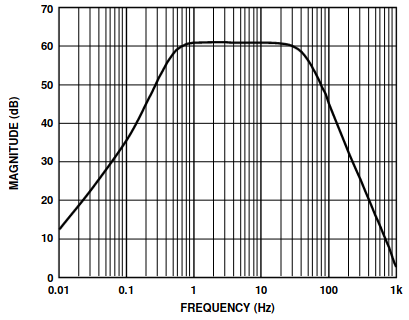
\includegraphics[scale=0.75]{pl/media/afilt.png}
    \caption{Wykres charakterystyki częstotliwościowej zastosowanego układu filtrów analogowych podany przez producenta \cite{AD8232ds}(\textit{Fig. 67.})}
    \label{fig:afilt}
\end{figure}

\newpage

\section{Próbkowanie, kwantyzacja i komunikacja z komputerem PC}

Do próbkowania i kwantyzacji sygnału zastosowano wbudowany w układ scalony mikorkontrolera \textit{STM32F411CE} przetwornik analogowo/cyfrowy o rozdzielczości 12 bitów \cite{STM32F4DS}.
Na podstawie literatury \cite{Ajdaraga2018} ustalono, że częstotliwość próbkowania $f_{s}$ o wartości $360 Hz$ dla sygnału \textit{EKG} spełnia zarówno założenia twierdzenia o próbkowaniu
jak i wymagania diagnostyczne.


W pracy użyto wbudowanego w \textit{STM32F411CE} kontrolera \textit{DMA} (\textit{Direct Memory Access}), umożliwiającego
transfery danych między przetwornikiem \textit{ADC} a pamięcią \textit{SRAM} w sposób niezależny od rdzenia mikrokontrolera. 
Umożliwiło to równoległe przetwarzanie danych trafiających do bufora przez rdzeń \textit{ARM Cortex M4}. 
Próbkowanie z częstotliwością $f_{s}$ zrealizowano za pomocą wbudowanego
układu licznika cyfrowego w konfiguracji generującej przerwanie co okres $T_{s} = \frac{1}{f_s}$, każde przerwanie rozpoczyna kolejną konwersję przetwornika
\textit{ADC} oraz następujący po nim transfer próbki poprzez \textit{DMA}.
\textit{STM32F411CE} posiada rdzeń procesora \textit{ARM Cortex M4} który w swojej architekturze 
(\textit{ISA}, \textit{Instruction Set Architecture}) zawiera również instrukcje użyteczne w cyfrowym przetwarzaniu sygnałów (\textit{DSP}, \textit{Digital Signal Processing}) \cite{CM4DSP} takie jak na operacje na liczbach zmiennoprzecinkowych czy
instrukcje typu \textit{SIMD} (\textit{Single Instruction Multiple Data}).


Komunikację z komputerem PC zrealizowano za pomocą interfejsu \textit{UART} (\textit{Universal Asynchonous Receiver/Transmitter}). 
Wbudowany w programator \textit{ST Link} układ mostka \textit{UART/USB} umożliwił komunikację z użyciem \textit{UART} poprzez fizyczny interfejs \textit{USB} w komputerze PC.
W celu zapisu i podglądu sygnału zaprojektowano i zaimplementowano aplikację okienkową na system operacyjny \textit{GNU/Linux} 
dla architektury standardowych komputerów klasy PC (\textit{x86\_64}).
Na potrzeby aplikacji zaprojektowano również odpowiedni protokół komunikacyjny w celu zapewnienia możliwości 
konfiguracji urządzenia oraz odczytywania próbek w ujednolicony sposób. 
Aplikację zaprojektowano z myślą o komunikacji ze sprzętem poprzez standardowe sterowniki 
np. \textit{cdc\_acm} \footnote{\url{https://github.com/torvalds/linux/blob/master/drivers/usb/class/cdc-acm.c}}
dla systemu \textit{Linux} w wersji \textit{6.5}.

